\documentclass[acmtog]{acmart}
\usepackage{graphicx}
\usepackage{subfigure}
\usepackage{natbib}
\usepackage{listings}
\usepackage{bm}
\usepackage{amsmath}

\definecolor{blve}{rgb}{0.3372549 , 0.61176471, 0.83921569}
\definecolor{gr33n}{rgb}{0.29019608, 0.7372549, 0.64705882}
\makeatletter
\lst@InstallKeywords k{class}{classstyle}\slshape{classstyle}{}ld
\makeatother
\lstset{language=C++,
	basicstyle=\ttfamily,
	keywordstyle=\color{blve}\ttfamily,
	stringstyle=\color{red}\ttfamily,
	commentstyle=\color{magenta}\ttfamily,
	morecomment=[l][\color{magenta}]{\#},
	classstyle = \bfseries\color{gr33n}, 
	breaklines=true, 
	tabsize=2
}
\lstset{basicstyle=\ttfamily}

% Title portion
\title{CS171 Final Report:\\ {Multi-Resolution Isosurface Rendering}} 

\author{
	Group Number:\quad 1 \\
	Member 1:\quad Hui Ren\\
	Member 2:\quad Yian Li\\
	Member 3:\quad Haiyu Song
}

% Document starts
\begin{document}


\maketitle


\vspace*{2 ex}


\section{Introduction}


This project required us to render iso-surface according to given data in vdb files which has multi resolutions based on ray-tracing techniques. Since the data is the air flow vector of a moving ball in the air, we using Q-criterion value for sampling and transfer, which visualize eddy detail of air. According to the reference paper, we implemented KD-tree for multi-resolution space searching and interpolation, analytic gradient for lighting, adaptive sampling and so on. \\
In implementation, we also met some problem tried to solve them. First we found it is hard for ray-tracing based iso-surface rendering between multi-resolution grid. Second we found the adaptive sampling paper introduced is not perfect. Additionally, we use binary search between small and large value points to subdivision the interval to sampling thus avoiding missing needed points, which highly speeds up performance.


\section{Background}


In this project, we need to render multi-resolution isosurface based on ray tracing. The paper "Ray Tracing Structured AMR Data Using ExaBricks"  we referred has some key contributions: \\
First, it gives a new data structure to organize AMR data(Adaptive Mesh Refinement) which supports high-quality cell interpolation, including across level boundaries. \\
Second, it gives out a novel analytic method to compute gradient vectors from reconstruction samples, which speed up computation.  \\
Third, it gives an adaptive sampling and opacity correction method for adaptive sampling.\\
Fourth, it contributes a thorough evaluation on realistic models and rendering methods.


\subsection{Active Brick Regions structure}
Given an AMR data, the paper first convert it to a new data structure which has many advantages. To do this, paper defines three concepts first:\\
1. Cell. It is the smallest unit in the data structure. First we have a smallest side length(finest) in the world. The cells with finest side length is with level 0, and the cells of next level 1 have 2 times of level 0, and so on. The neighbor cells will have level difference at most 1, so that cells with different size will be aligned. So that each cell has a int coordinate which can indicate its world position. 
2. Brick. A brick is a box that is filled with cells of same level. For a brick, its coordinate is defined as the coordinate of the left-bottom cell in it. It also contains the level information of cells in it.
3. Support. A support is bind to a brick and larger than the brick, which is a region of space where the sample reconstruction function is non-zero. Its function is to provide convenience for interpolation and KD-tree partition.
Then we know supports may have overlaps. Each overlap forms a spatial partition and tells we what bricks are "active" in that region of space. i.e. At least one cell from these bricks has non-zero contribution in the region.
\begin{figure}[h]
	\centering	
	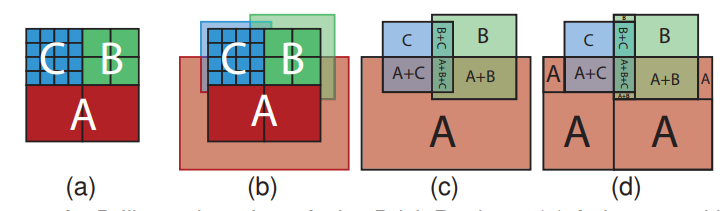
\includegraphics[width=0.7\linewidth]
	{images/ABR.png}
	\caption{A 2D Illustration of our Active Brick Regions}
\end{figure}

Like the picture, the supports and their overlap forms a partition of space, and each region tells the contributions of bricks(A,B,C).\\
Then we can do KD-tree construction from these supports. In this project the given input files has multiple "grids", which corresponding to "support" concept there.

\subsection{Adaptive sampling and opacity correction}
A simple way to do adaptive sampling is to just take the side length of current cell while ray tracing. However, as paper introduces, this will generate terrible aliasing on region boundaries when regions are sampled at different rates. So the paper take original adaptive sampling positions as delimiters of sub-intervals and take mid-points as actual sample position. The length of these intervals are used as weights for opacity correction.\\
At first we tried the way paper introduced. However, we found that it is not very well when it comes to rendering iso-surfaces with very thin thickness, such as under Q-criterion. Only when step scale is very small, such as 0.01, the result can converge to an acceptable result, but this will lead to high time cost.\\
Instead we use a new advanced adaptive sampling method, which will be introduced following. Even when step scale is 0.5, the result is acceptable, and only cost a little time. 

\subsection{Gradient vectors}
The normal way to get gradient vectors for iso-surfaces is by central differencing. However, for ray-tracing based method, this will \\
\\
\\
be every slow. The paper gives out an analytic way to get the gradients, which has obvious performance promotion and little quality sacrifice.



\subsection{Reconstruction filter}
The normal way to do the reconstruction is using nearest-neighbor reconstruction. However, it has obvious limitations in terms of image quality, in particular for spiky transfer functions and iso-surfaces. So the paper use another reconstruction way to do this.


\section{Methodology and Implement}


\subsection{VDB file load}


Since the input files given are .vdb files, we should first load it in using openvdb lib. Each grid has its dx, origin information. The original data is a vector field data, stored in local coordinate in each grid. The transform function defined in the file gives out the mapping relation between coordinate and world position, it provides convenience for interpolation afterwards.\\
Then we compute q-criterion value and vector norm of grid cell vertices. Q-criterion will be using for transfer function, and normal value will be use in color mapping, so the eddy detail will be visualized clearly.


\begin{figure}[h]
	\centering	
	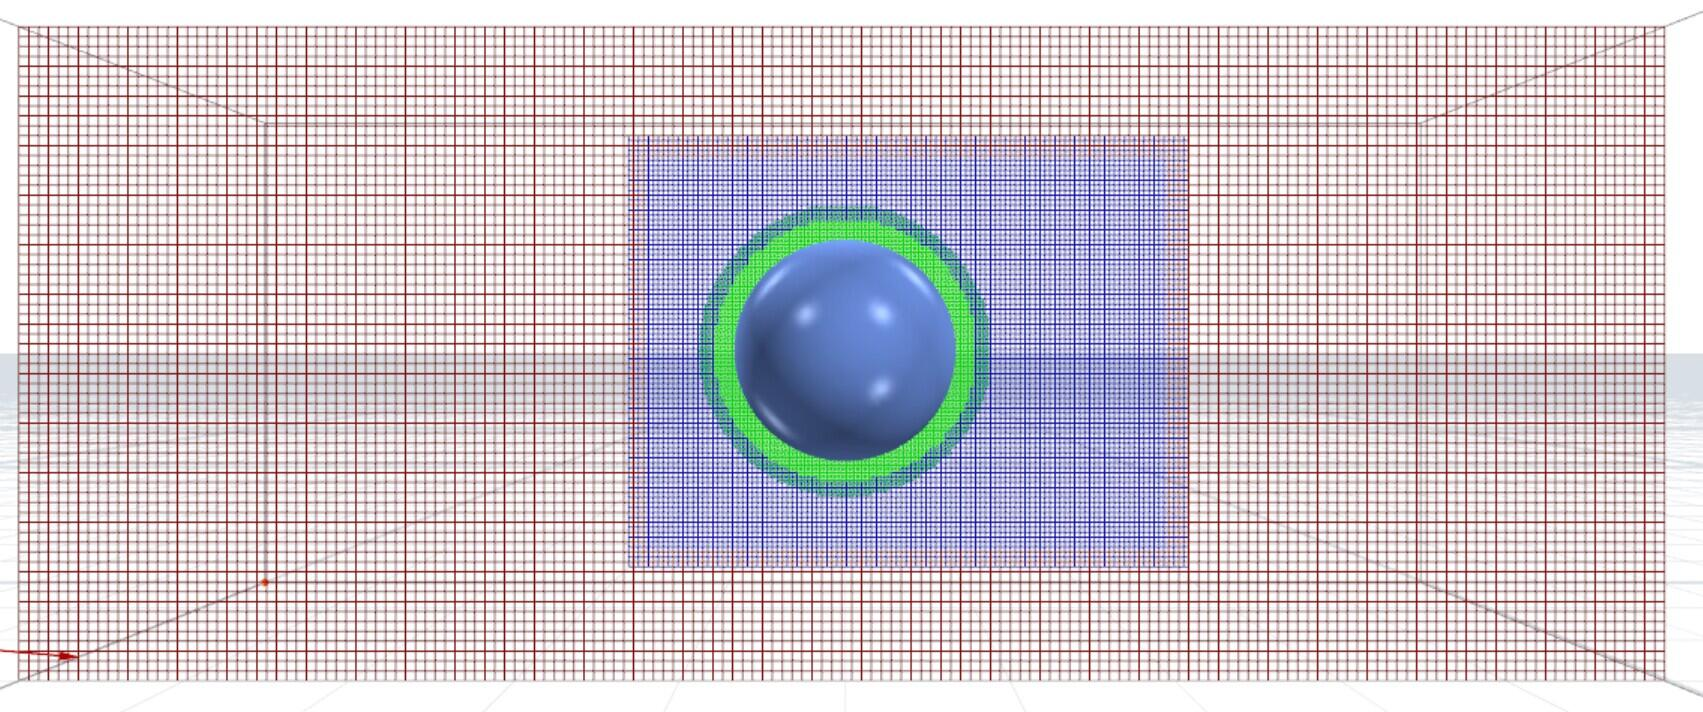
\includegraphics[width=0.7\linewidth]
	{images/data.jpg}
	\caption{The format of the readin data}
\end{figure}


\subsection{Front to back composition}


Given a position in the world, we can first get its value by searching kd-tree and return corresponding contribute grids. Then we choose the finest contribute grid and do interpolation in it to get the value of this point. Then we can get its opacity(from transfer function), and color (color mapping). We can then add its radiance contribution to the corresponding pixel using front-to-back method. Viewing rays are traversed from camera into the volume, we have:
\begin{figure}[h]	
	\centering	
	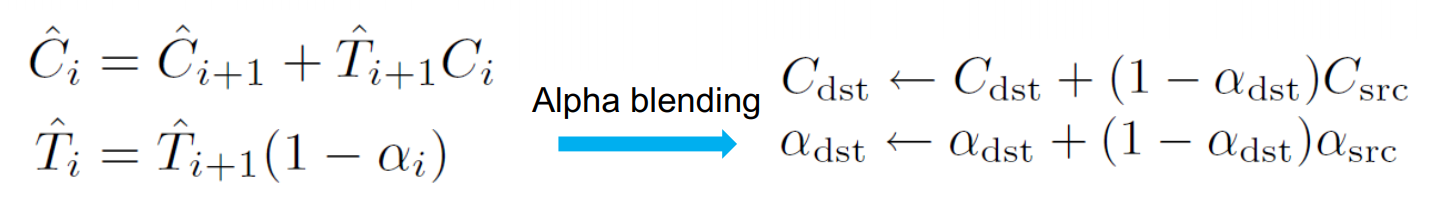
\includegraphics[width=0.8\linewidth]
	{images/f-1-20-26.png}
	\caption{Front to back composition}
\end{figure}
The equation saves opacity results, while we save transparency result(1-opacity) equally for easier understanding, which is 1 at first. For example, when tracing at a point, we have global T, color result C, the transparency $T'$ for this point, and $C'$ for its color. Notice our color map does not contain transparency, we should first update C, as $C'*=T'$, then $C=+=T*C'$ and $T*=T'$.\\
At the beginning of tracing, we first decide whether it intersects with a bounding box in the scene, if yes, we get the tracing range for the ray and tracing from the position where ray goes into the bounding box. When tracing, if T becomes every small, near zero, which means the ray becomes dim, the tracing ends.


\subsection{pre-integration}
The classic interpolation-based transfer function consists of two
techniques introduced in popular ways, namely post-integrated transfer functions and 
pre-integrated transfer functions.\\
The former is the same as interpolating in the raw data of the data value, and then use 
the transfer function to convert it. The latter is equivalent to converting the raw 
value of the data to process the information and then pass information processed.\\
In general, the pre-integral transfer function produces a smoother one
results and avoid aliasing.\\


\subsection{Q criterion}
Q-Criterion is an important calculation used to identify vortices.\\
The value Q comes from the definition of the velocity gradient tensor $\delta_{Ui}/\delta_{Xj}$ which can be 
broken out into two parts such that:
$$\delta_{Ui}/\delta_{Xj}=\frac{1}{2}((\delta_{Ui}/\delta_{Xj})+(\delta_{Uj}/\delta_{Xi}))+
\frac{1}{2}((\delta_{Ui}/\delta_{Xj})-\delta_{Uj}/\delta_{Xi})$$
where the symmetric part will be denoted as $S$ and is known as the strain rate tensor defined by"
$$S=\frac{1}{2}((\delta_{Ui}/\delta_{Xj})+(\delta_{Uj}/\delta_{Xi}))$$
and the anti-symmetric part denoted as $\Omega$ is known as the rotation rate or voracity tensor 
defined by:
$$\Omega=\frac{1}{2}((\delta_{Ui}/\delta_{Xj})-\delta_{Uj}/\delta_{Xi})$$
And the viscous stress tensor defined as:
$$\tau =\mu((\delta_{Ui}/\delta_{Xj})+\delta_{Uj}/\delta_{Xi})$$
we see that the viscous stress are specifically functions of the strain rate only.\\
Q is defined as the second invariant of the velocity gradient tensor
$$\begin{aligned}
	Q&=\frac{1}{2}(||\Omega||_F^2-||S||_F^2)\\
	&=-\frac{1}{2}((\frac{\partial u}{\partial x})^2+(\frac{\partial v}{\partial y})^2+
	(\frac{\partial w}{\partial z})^2)-\frac{\partial u}{\partial y}\frac{\partial v}{\partial z}-
	\frac{\partial u}{\partial z}\frac{\partial w}{\partial x}-\frac{\partial v}{\partial z}\frac{\partial w}{\partial y}
\end{aligned}
$$
Having the pesudocode as follow:
%\textcolor{blue}{Pesudo Code}
\begin{lstlisting}
	[dudx,dudy,dudz] = gradient(ux);
	[dvdx,dvdy,dvdz] = gradient(uv);
	[dwdx,dwdy,dwdz] = gradient(uw);
	Q=-0.5*(dudx.^2+dvdy.^2+dwdz.^2)
	-dudy.*dvdx-dudz.*dwdx-dvdz.*dwdy;
\end{lstlisting}


\subsection{The interpolation method}


Since, nearest neighbor reconstruction has obvious limitations especially for spiky transfer functions and iso-surfaces. High-quality rendering requires the use of a more advanced reconstruction filter. In our project, we choose to use the basis method by Wald et al. for reconstruction, which is also the interpolation method choose by the paper "Ray Tracing Structured AMR Data Using ExaBricks" we reproduced.


Regular trilinear interpolation can also be viewed as the sum of 8 hat-shaped basis functions located at the dual cell’s corners:
\[\mathrm{lerp}(\vec{P},D)=\sum_{C\in corners(D)}\hat{H}_{C}(\vec{P})C_{v},\]
using the hat-shaped basis functions:
\[\hat{\mathrm H}_{C} (\vec{P}) = \hat{h}\left(\frac{|\vec{C_{p,x}}-\vec{P}_{x}|}{C_{w}}\right) \hat{h}\left(\frac{|\vec{C_{p,y}}-\vec{P}_{y}|}{C_{w}}\right) \hat{h}\left(\frac{|\vec{C_{p,z}}-\vec{P}_{z}|}{C_{w}}\right),\]
with $\hat{h}(t) = \text{max}(1 - t, 0)$. For each cell C this basis function would be centered at $C_p$ and have a support width of $\pm C_w$.


Reconstructing a sample at position $\vec{P}$ then involves finding all cells $C_i$ with data value $C_{vi}$ that have non-zero support $\hat{H}_{C_i}(\vec{P})$ and computing the weighted sum:
\[B(\vec{P})=\frac{\sum_{C_{i}}\hat{H}_{C_{i}}(\vec{P})C_{vi}}{\sum_{C_{i}}\hat{H}_{C_{i}}(\vec{P})}\]


Having the pseudocode from the original paper:
\begin{lstlisting}
float sum_weights = 0
float sum_weightedValues = 0
for (l = 0...)
	D = findDualCell (P)
	foreach corner cell C of D
		if (C is a leaf cell)
			sum_weights += H_hat (P, C)
			sum_weightedValues += H_hat (P, C)*C_v
	if (none of the C in D are inner nodes)
		break
return sum_weightedValues / sum_weights
\end{lstlisting}


\subsection{Adaptive sampling}


\subsubsection{1. Tring paper's method}


As in background part, just take side length of finest contribute grid of current point is not good. So we first take original adaptive sampling positions(step scale * cell side length) as delimiters of sub-intervals and take mid-points as actual sample position. The length of sub-intervals is used as weights to do opacity correction.


\begin{figure}[h]	
	\centering	
	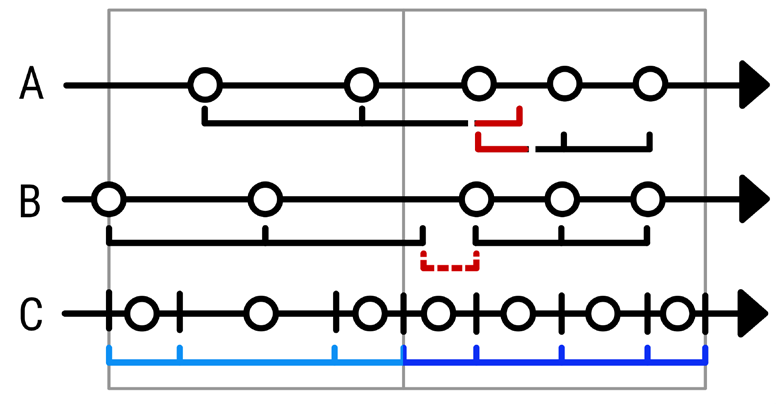
\includegraphics[width=0.8\linewidth]
	{images/adaptive.png}
	\caption{Adaptive sampling}
\end{figure}
Like the picture, if successive regions are sampled at different rates, the distance between the last sample in one and the first sample in the next can be samller(A) or larger (B) than either region's sampling rate. This leads to artifacts on the boundaries. After our operation, the actual sample points like (C) shows.


However, when we use Q-criterion, we found that in a cell the eight vertices will very likely to have very difference values. So the interpolation values in the cell will have drastic change, which means the iso-surface can be very thin. It is hard for rendering iso-surface because the ray will likely to go through the wanted surface without sampling it. Only when step scale is very small, the result can have a better quality. We tried the step scale until 0.01, which gives out a acceptable result, but it is very time-consuming, which is not acceptable. So we tried another way.


\subsubsection{2. Advanced adaptive sampling}


The thing to optimize is how to add sample points near the iso-surface so that the ray will unlikely to be under-sample. 


For rendering iso-surface, the trensfer function we defined has an interval around the iso-value in which the opacity got is non-zero.


First we define three sample status: in interval(0), smaller than interval(1), greater than interval(2).\\
The initial sample position chosen is the same as the paper does, i.e. take the mid-point of sub-intervals. Then we judge the sample status of this point, if it is 0, then just take this point and compute its radiance contribution. Then if it is 1, but last one is 2, or it is 2 but last one is 1, which means there might be a suitable point should be taken between these two points. Then we do binary search in this interval to find if there has one. If yes, then sample points will be changed to it. And if last one is 0, then this point will be taken for further searching.
This method is based on the principle that interpolation is continuous.\\
The weight of opacity correction is taken as the space distance between current sample point and the last one, which is more reasonable.\\
The last thing is about searching depth, it should not be too deep or the performance will be influenced. In former trying we found that when step scale<=0.01 will have a good result. To let the final interval during searching to become this, we set the depth to: $log_2(\frac{step\_scale}{0.005})$.\\
What's more, we have done interleaved sampling where ray first goes into the bounding box: $t_0=dt(\rho + \lceil \frac{t_0+\rho dt}{dt}\rceil)$. Where $\rho$ is a per-ray random offset for interleaved sampling, and dt is the scaled base sampling step.\\
Doing this, even when step scale is 0.5, the result is still acceptable, and performance is still good, with speed like just normal adaptive sampling with step scale of 0.5.\\
\\
\\
\\
\subsection{Transfer function and parameters(Opacity transfer)}


In order to rendering a specific isosurface, we designed an opacity transfer function. The opacity is determined by the q criterion of the given position. Taking the isosurface with isovalue = 0.05 as an example, we have the following opacity transfer function:
\begin{align*}
	\text{Opacity}(val) = \begin{cases}
		\text{min}(1, 1.6*\exp(-0.5*(x - 0.05)^2 / 0.004^2)), \\
		\quad \quad \quad \quad \quad \quad \quad \quad \text{for }x \in (0.042, 0.058)\\
		0, \text{elsewhere}
	\end{cases}
\end{align*}
and having the plot as follow:
\begin{figure}[h] 
	\centering	
	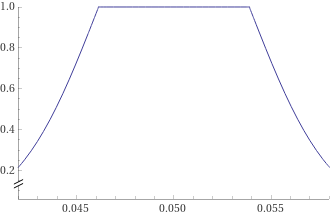
\includegraphics[width=0.6\linewidth]{images/opacity.png}
	\caption{Transfer function}
\end{figure}\\
its support is from 0.042 to 0.058.


The reason we designed the the shape of the opacity transfer function in this way is that the change in q-criterion is continuous, but the front-to-back volume rendering method we use only samples for discrete picking points, so we need to set the opacity in an interval to be 1. When our discrete sampling points encounter any of the values in that interval, they are considered to be the iso-surface we need to render. Around the very small interval of 0.004 that we defined, we also added a Gaussian kernel in order to increase the robustness of the sampling, when encountering the value of the dramatic changes, it is difficult to sample the exact position of the given isovalue, by adding a certain translucent area, as far as possible to restore the actual iso-surface.


\subsection{Opacity correction}


Since the dx in the given VDB data is different in different grids, and also we use adaptive sampling, the step size is different each time. 


The assigned opacity depends on the specific sampling rate. For example, when using fewer slices, the opacity has to be scaled up, so that the overall intensity of the image remains the same. Using the formula below to correct the transfer function opacity whenever the user changes the sampling rate $\Delta x$ from the reference sampling rate $\Delta x_0$:
\[\alpha_{corrected} = 1 - [1 - \alpha_{stored}]^{\Delta x / \Delta x_0}\]
To control the quality and speed of rendering, we can change the maximum number of slices i.e. $\Delta x / \Delta x_0$ from the user interface we designed.


\subsection{Color mapping}


We designed our own color transfer function in order to better showing the rendering results. On an isosurface, the q criterion are the same, but the speed(norm) of the air are different. We will establish a mapping from the speed(norm) of the air to the RGB color for the color matching. Considering that we have designed the user interface, in the user interface we can define any number of air speed values with a specific color, and within a small neighborhood around the defined value, the isosurface will be directly assigned the set value. In other areas, we do linear interpolation between the two endpoints of the interval to get the color corresponding to each speed value.


In detail having three basic rules for color matching:
\begin{itemize}
	\item For the interval of 0.0025 before and after the speed value of the set color, that is, the interval of 0.005 in total, the color of this point is assigned i.e. 0.4, red -> 0.375~0.425, red\\
	\item For the value between two intervals, linear interpolate\\
	\item For the value that is smaller than the set point with the smallest value or larger than the set point with the largest value, the value is directly assigned according to the color of the set minimum value point or maximum value point
\end{itemize}


\subsection{Gradient}


For the basis reconstruction method we used, it is actually possible to compute the gradient analytically. Which means that the gradient of the given position can be computed simply using the existing data values loaded for the original sample evaluation, without additional memory accesses or ray traversals. The gradient can be computed as the first order partial derivatives as definition(taking the gradient on x-axis as example, other two directions are same):
\[
\frac{\partial{B(p)}}{\partial x} = \frac{\sum_{C}\hat{H}_{C}(p)\sum_{C} \frac{\partial\hat{H}_{C}(p)}{\partial x}C_{v} - \sum_{C}\hat{H}_{C}(p)C_{v} \sum_{C}\frac{\partial\hat{H}_{C}(P)}{\partial x}}{()\hat{H}_{C}(p))^{2}}.
\]
The gradient of $\hat{H}_C (p)$ can be easily calculated as,
\[
\frac{\partial\hat{H}_{C}(p)}{\partial x}}=\hat{h}\left({\frac{|C_{p y}-p_{y}|}{C_{w}}}\right)\hat{h}\left({\frac{|C_{p z}-p_{z}|}{C_{w}}}\right)\chi(x){\frac{1}{C_{w}}
\]
where $\chi(t) = 1$ if $p_t > C_{pt}$ and $\chi(t) = 1$ elsewhere.


Repeat the above process for three time and we will get a 3 dimension vector, which is the gradient for the given position on the isosurface, we will use this when applying phong lighting for the isosurface.


\subsection{KD tree construction}


Since the input data are vdb files, which already gives us "support", the function for the kd tree is: given a world position, it should return which grids contribute to it, so that we can to interpolation on the position. So for each tree node, we save the partition axis, partition position, and contribute grids. We use a greedy method to construct the KD-tree:


\begin{figure}[h]
	\centering
	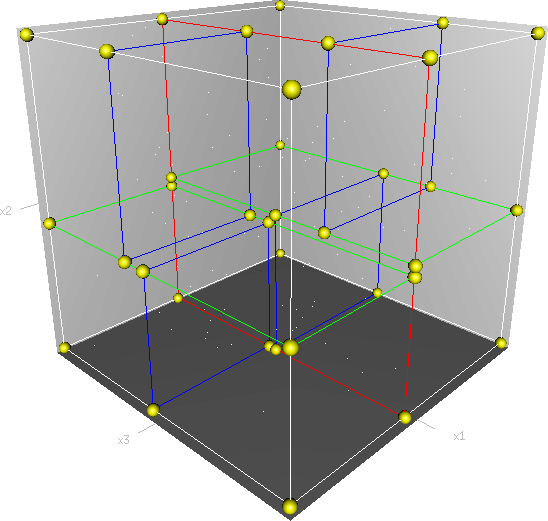
\includegraphics[width = 0.5\linewidth]{images/kdtree.jpg}
	\caption{The KD tree structure}
\end{figure}


At first, it is easy to get the whole bounding box, and bounding boxes for each grids. The contribute grids for the root node is just all the grids. Then we choose the longest axis as partition axis. For example, the axis we choose is x axis now. Then, for each other bounding boxes, we can get two position of this axis(min and max). We put these positions in a vector and then do sort operation, and choose the middle one as partition position.


Observe that, for each bounding box of contribute grids now, if the min position on the partition axis is larger than partition position, it means left child will not have this contribute grid any longer. For right, it is the same, if a max position of a grid bounding box is smaller than partition position, it means right child will not have its contribution any longer. This operation we use std::set to store temp positions and to iterate, so that the construction speed can be fast. Then the original bounding box will be split according to partition position to create both children.


When construction grids remain only one, the construction will stop. We tried if limiting the depth of tree will have influence on following tracing speed. We found that, for given data, limiting depth to <=8 will have the best performance. Furthermore, we think when given a lot of grids, and depth becomes large, there should be an obvious trade-off between depth(for searching) and contribute grids return(for interpolation).


What's more, using vector to store contribute grid is very costly. So we use bitmap to do this, which actually has remarkable performance improvement. Using a uint32\_t for bitmap, bit i (0 to 31) representing the grid i. For example, 0b0101 in bitmap representing grid 0 and grid 2 have contributions to the given area. Using bit operations, addition and subtraction can be much more efficiency then dealing with a int vector.


\subsection{Put object into the volume}


For the project we are required to load in an .obj file which stores sphere meshes and put it into the scene. Like homeworks before, it is easy to load and put it in the right place by using tinyobjloader lib.\\
Then we construct a BVH tree on the sphere for ray tracing, the detail implement method is described in the next part.\\
For each ray, it will first do intersection test with the meshes, and record information like hit position, normal, distance. In the tracing process, the distance will reduce by actual sample step and when it comes to zero, Phong lighting will be done and we take result as color of the point. Since the sphere is opaque, after done this the tracing process will stop.


\subsection{BVH}
A bounding volume hierarchy (BVH) is a tree structure on a set of geometric objects. 
All geometric objects, that form the leaf nodes of the tree, are wrapped in bounding 
volumes. These nodes are then grouped as small sets and enclosed within larger bounding 
volumes. These, in turn, are also grouped and enclosed within other larger bounding volumes 
in a recursive fashion, eventually resulting in a tree structure with a single bounding 
volume at the top of the tree. Bounding volume hierarchies are used to support several 
operations on sets of geometric objects efficiently, such as in collision detection and 
ray tracing.\\

To acceclerate intersection query, we use volume bounding hierarchy 
to help. Because it is tree structure and faster to reduce intersection test.\\
We want to Select a partition of primitives that doesn't have too
much overlap of the bounding boxes.\\
And the basic idea is: Pick the longest axis, and divide it equally.\\

For better query, we introduce SAH(surface area heuristic) which use the surface area to 
present the probability of ray intersection. \\
For a convex volume A contained in another convex volume
B, the conditional probability that a random ray passing
through B will also pass through A is:
$$p(A|B)=\frac{s_A}{s_B}$$
So the building tree part is obvious. We split the node with minimal cost.\\


\subsection{UI}
To make it more user friendly, we design a UI which has mutliple setting parameters such as: 
spp, step scale, iso value, different mapping colors and image saving for better interaction.\\
With it, we can use different transfer funcion and rendering the image with different isovalues 
and different colors.

\begin{figure}[h]
	\centering
	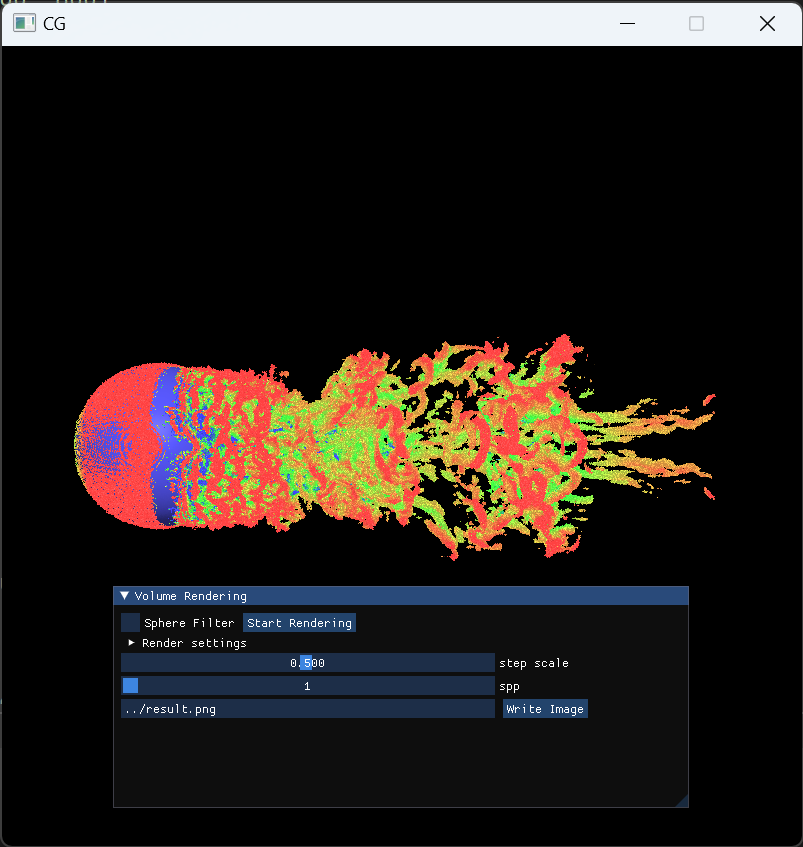
\includegraphics[width = 0.68\linewidth]{images/ui1.png}
	\caption{Basic setting}
\end{figure}
\ \\
\begin{figure}[H]
	\centering
	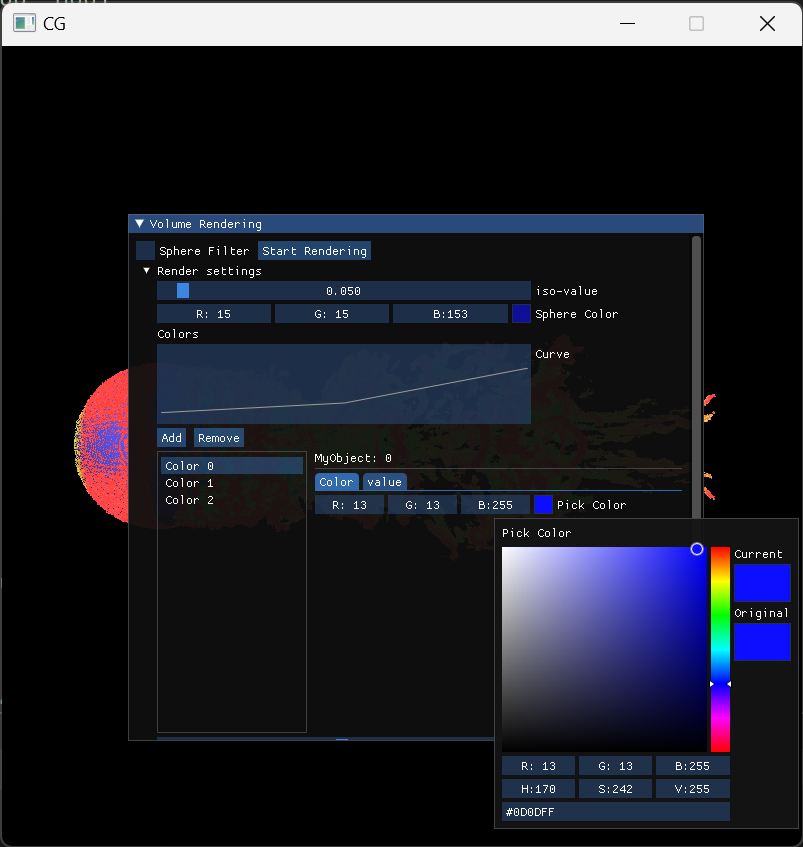
\includegraphics[width = 0.68\linewidth]{images/ui2.png}
	\caption{Parameter setting}
\end{figure}


\section{Problems and Future work}


\subsection{Q criterion discontinuity}


We found that for multi-resolution data, when we calculate the partial derivative of the speed change in each direction when calculating of the q criterion, using 2dx or dx (boundary) of the grid as the denominator, the obtained q value is discontinuous. It is especially obvious in the interval with a large value of q, especially the case of q > 0.6, as shown in the figure below.
\begin{figure}[h]
	\centering
	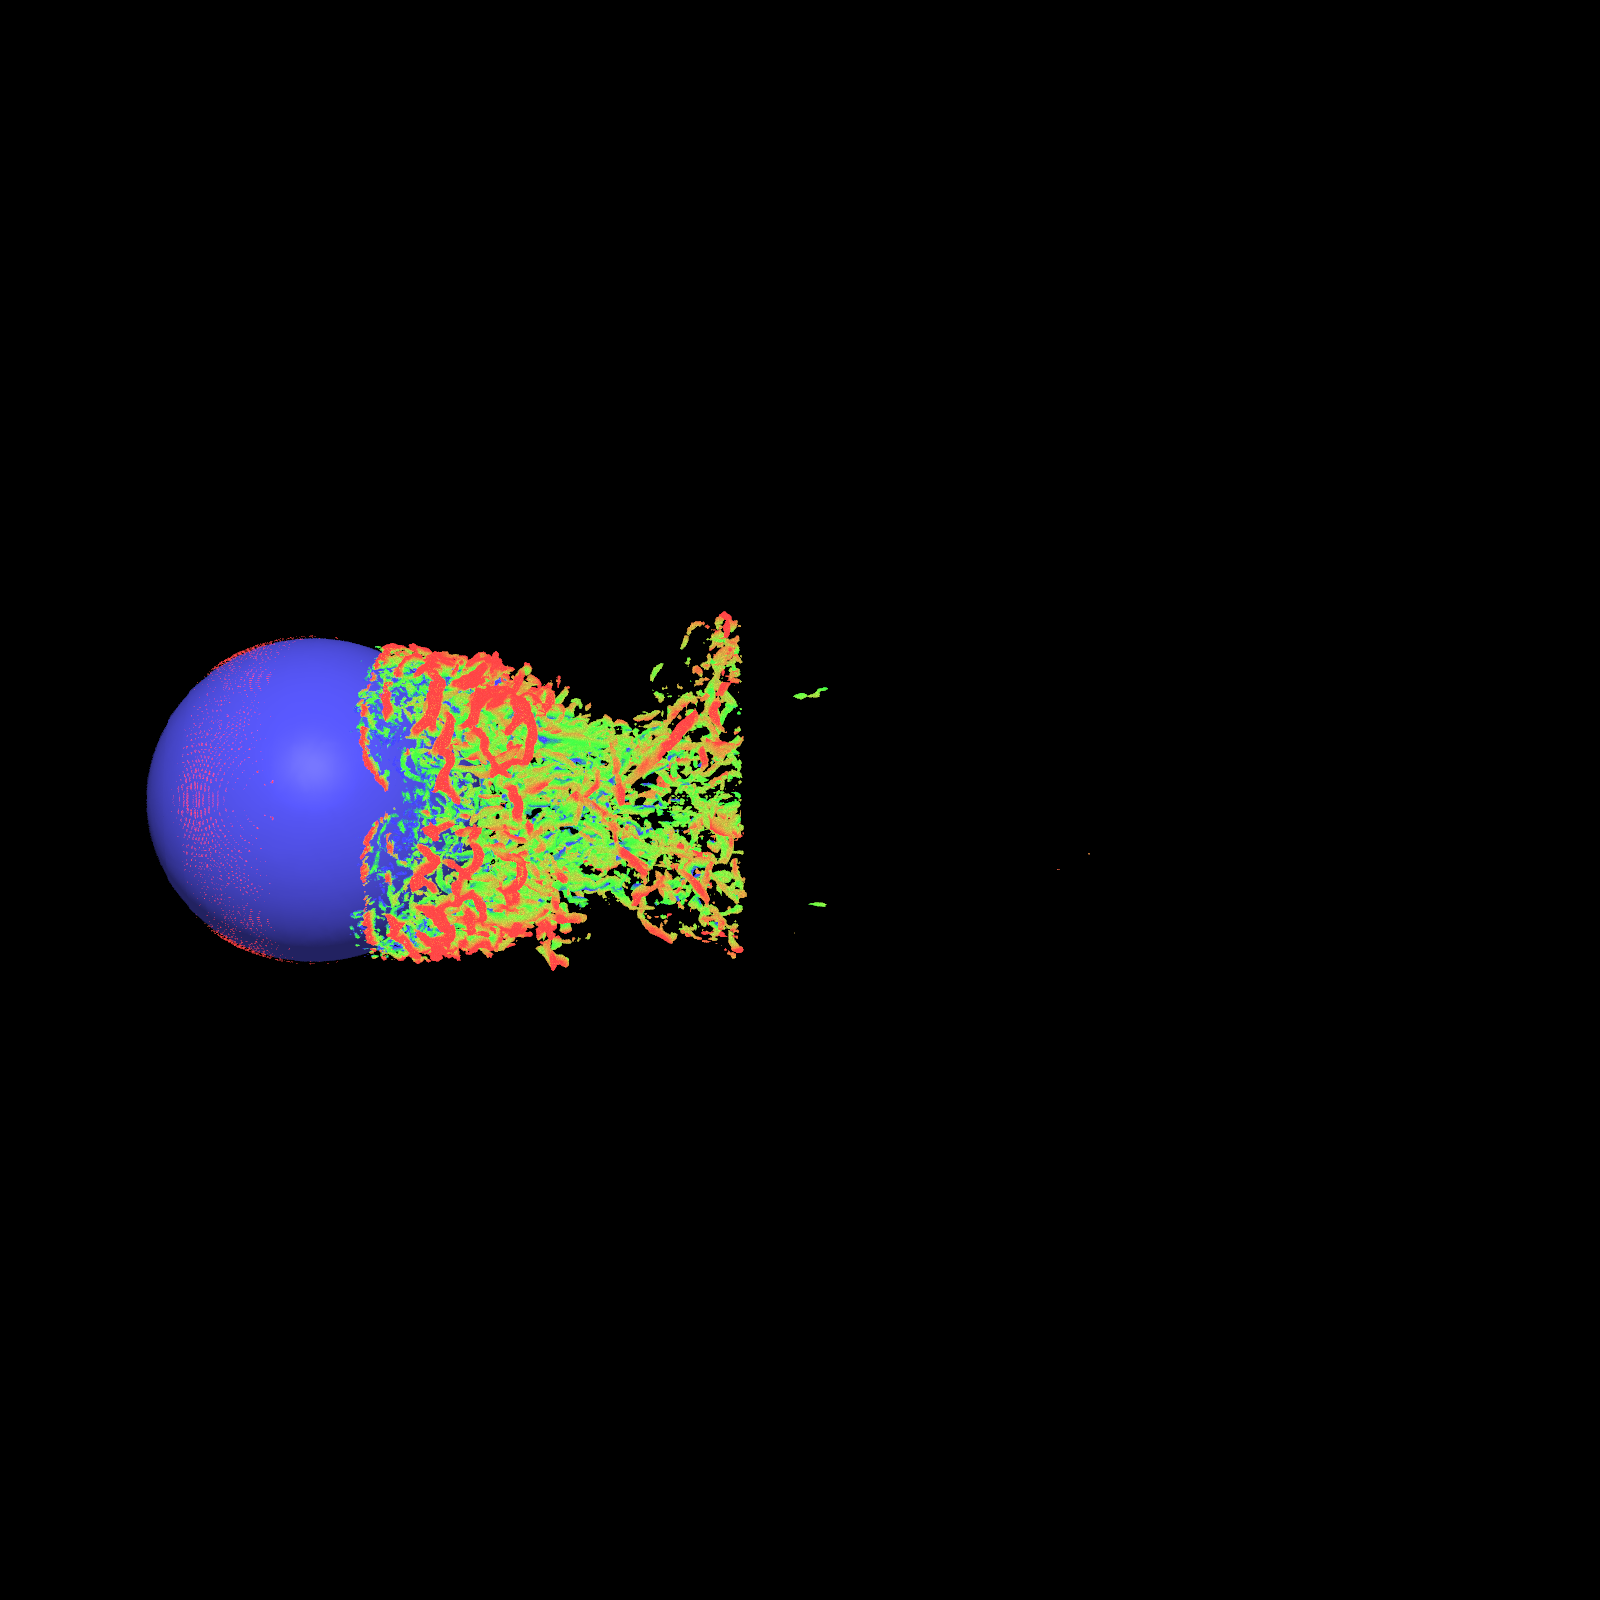
\includegraphics[width = 0.68\linewidth]{images/q-criterion.png}
	\caption{Q criterion is discontinue(isovalue = 0.65)}
\end{figure}


However, the strange thing is that when we use the same denominator for different resolution grids, we measure a large number of intervals and find that the q criterion values are continuous, but this is obviously wrong based on the definition of q criterion and partial derivative. This confused us, so we did a lot of experimentation and deep thinking, and we would like to thank the TA for kindly exploring this issue with us. We came to the following reasons.


Back to the definition of q criterion, it represent the the vorticity magnitude of a giving position. The q value of the vortex changes drastically at every location, both in direction and magnitude, especially in direction. When we perform q criterion calculation and interpolation calculation, we actually use the idea of ``'average'. For physical features that change drastically in direction, the ``'average' calculation is especially inaccurate for larger dx, so the details of turbulent flow cannot be guaranteed. When using a high q criterion, it is normal to be discontinuous at the boundary of the grid. The q criterion describes the details of the turbulence, so once the grid transition is involved and dx changed, the ``average'' area changed, the q criterion will change instantaneously, resulting in a discontinuous effect. Furthermore, why using the marching cube seems to have no problem on this issue, because the marching cube is a ``violent connection'', which guarantees that it must be connected algorithmically. 


Under the existing definition of q criterion and our rendering method of isosurface, this problem may be unsolvable. Perhaps we can only solve this problem by perfecting the definition of the q criterion, or using more advanced algorithms, which can be our future work.


\subsection{Cuda (nanovdb) problem}
In volume rendering, since we choose ray casting method, and use front to back rendering, rendering each 
pixel is relatively independent and the memory access don't have bank conflict. So, we can 
render the image in parallel theoretically.\\
\begin{lstlisting}
	dim3 dimGrid(width/TILE,height/TILE,1);
	dim3 dimBlock(TILE, TILE, 1);
	renderkernel<<<dimGrid, dimBlock>>>();
\end{lstlisting}
We assign pixels to CUDA thread, and for each thread, we use front to back rendering seperately 
and for data which frequently accessed, we can put it into shared memory.\\
For branches, we assign the thread with same condition to the same wrapper, 
thus can reduce performance loss.


However, $openvdb$ is kind of data structure and don't support CUDA. And we also failed to 
install $nanovdb$. In the future, we may use nanovdb with CUDA to acceclerate rendering and make it realtime.


\section{Results}


Run our code for rendering the iso-surface, and we get the following results. For all the results, we set three value-color pairs, and follow the linear color mapping method we introduced before. The three value-color pairs are: 0.012 -> {0.03, 0.03, 1.0}(B), 0.025 -> {0.03, 1.0, 0.03}(B), 0.072 -> {1.0, 0.03, 0.03}(R). All the result is rendered with isovalue = 0.05, the resolution is $1600 \times 1600$ with step length = $0.5 \times \mathrm{d}x$. Multi-big and single-big data have the rendered result shown below:


\subsection{Multi-big Data}


\begin{figure}[H]
	\centering
	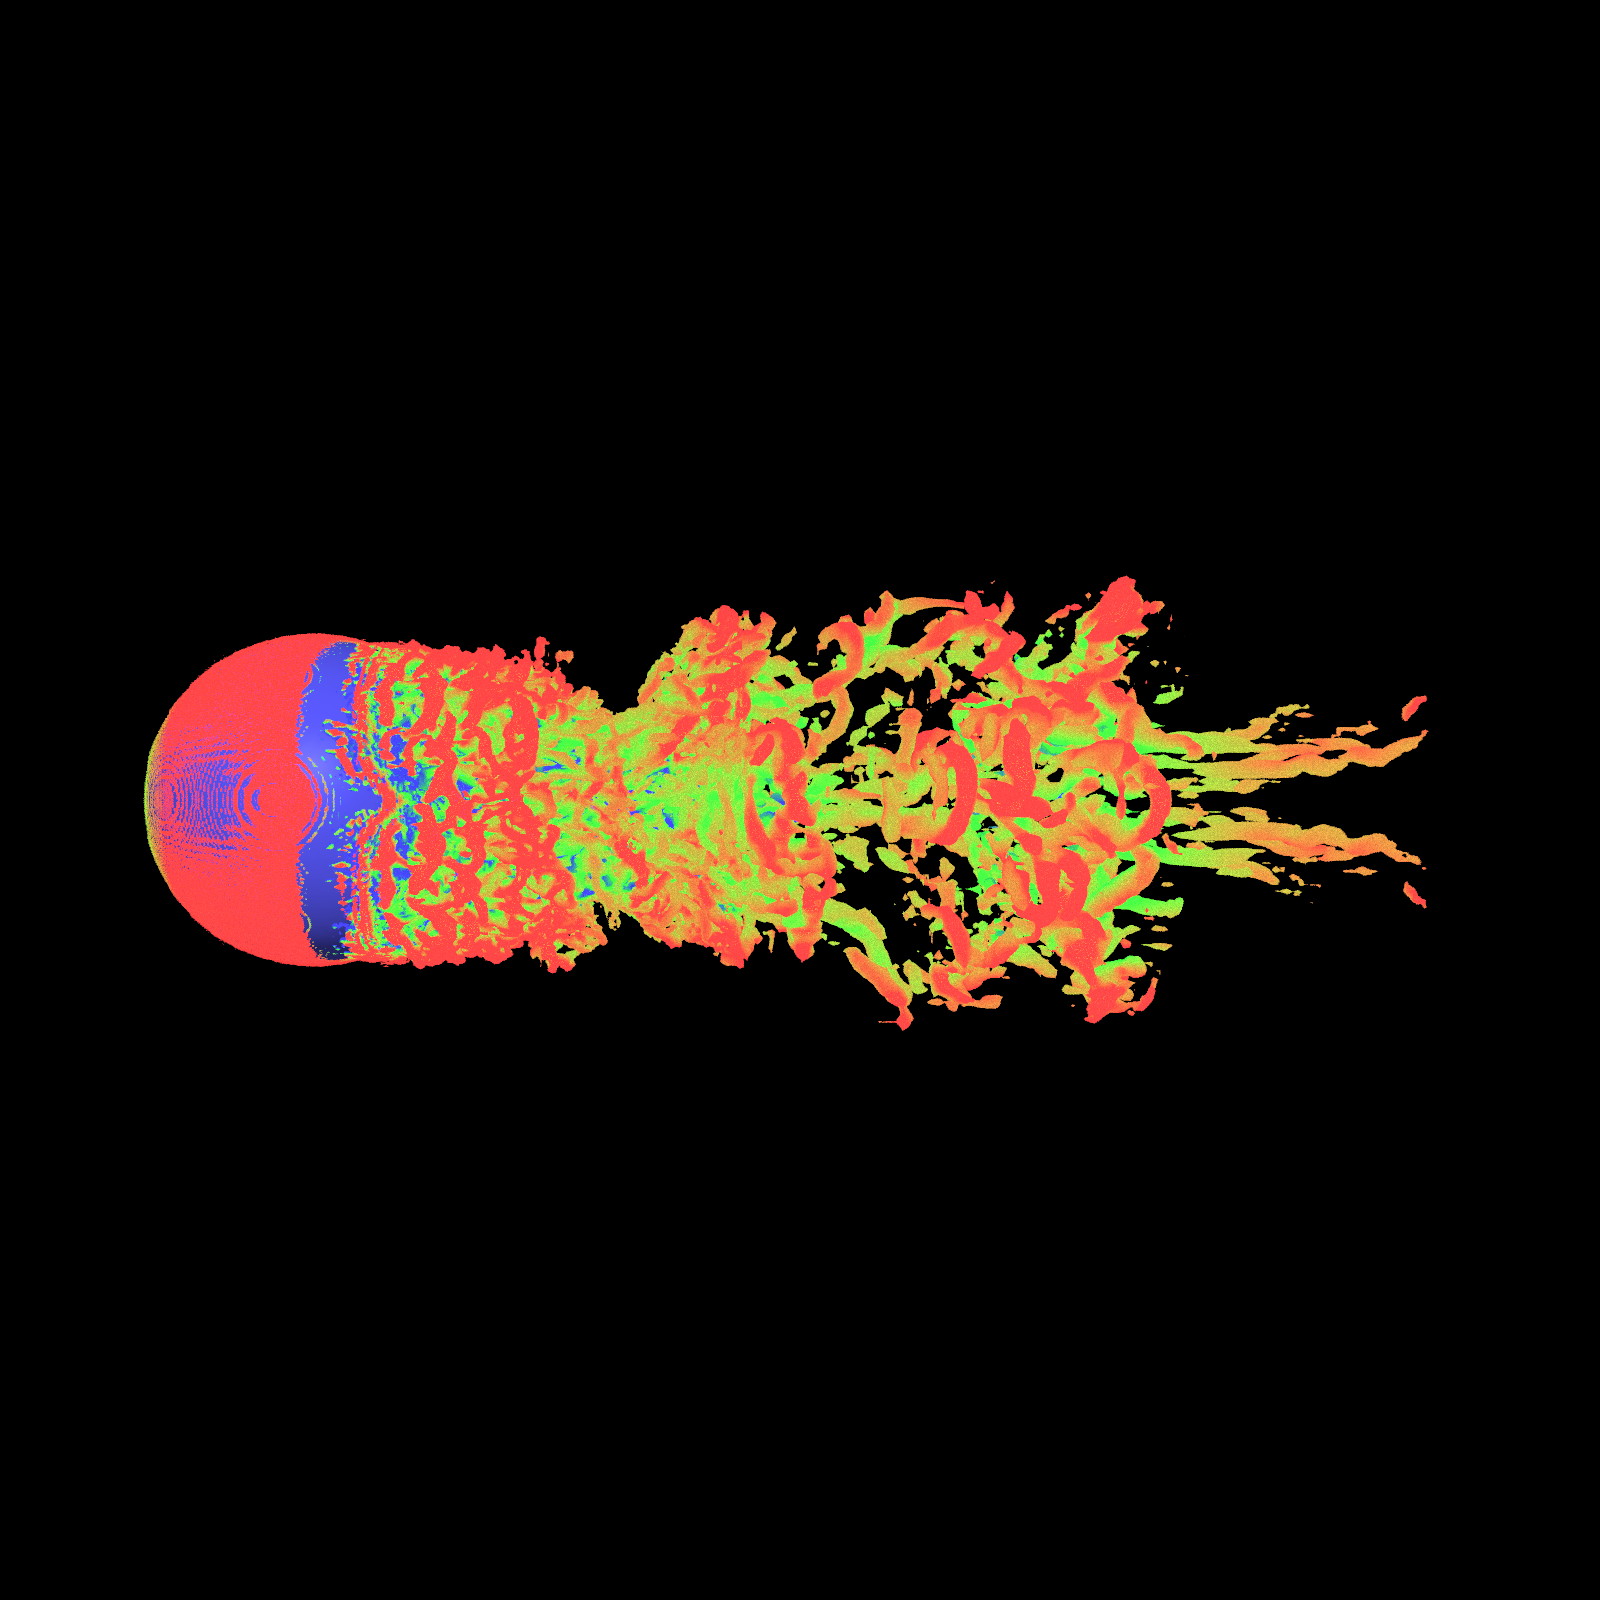
\includegraphics[width = 0.67\linewidth]{images/result_m_b_nf.png}
	\caption{Multi-big without filter}
\end{figure}
\begin{figure}[H]
	\centering
	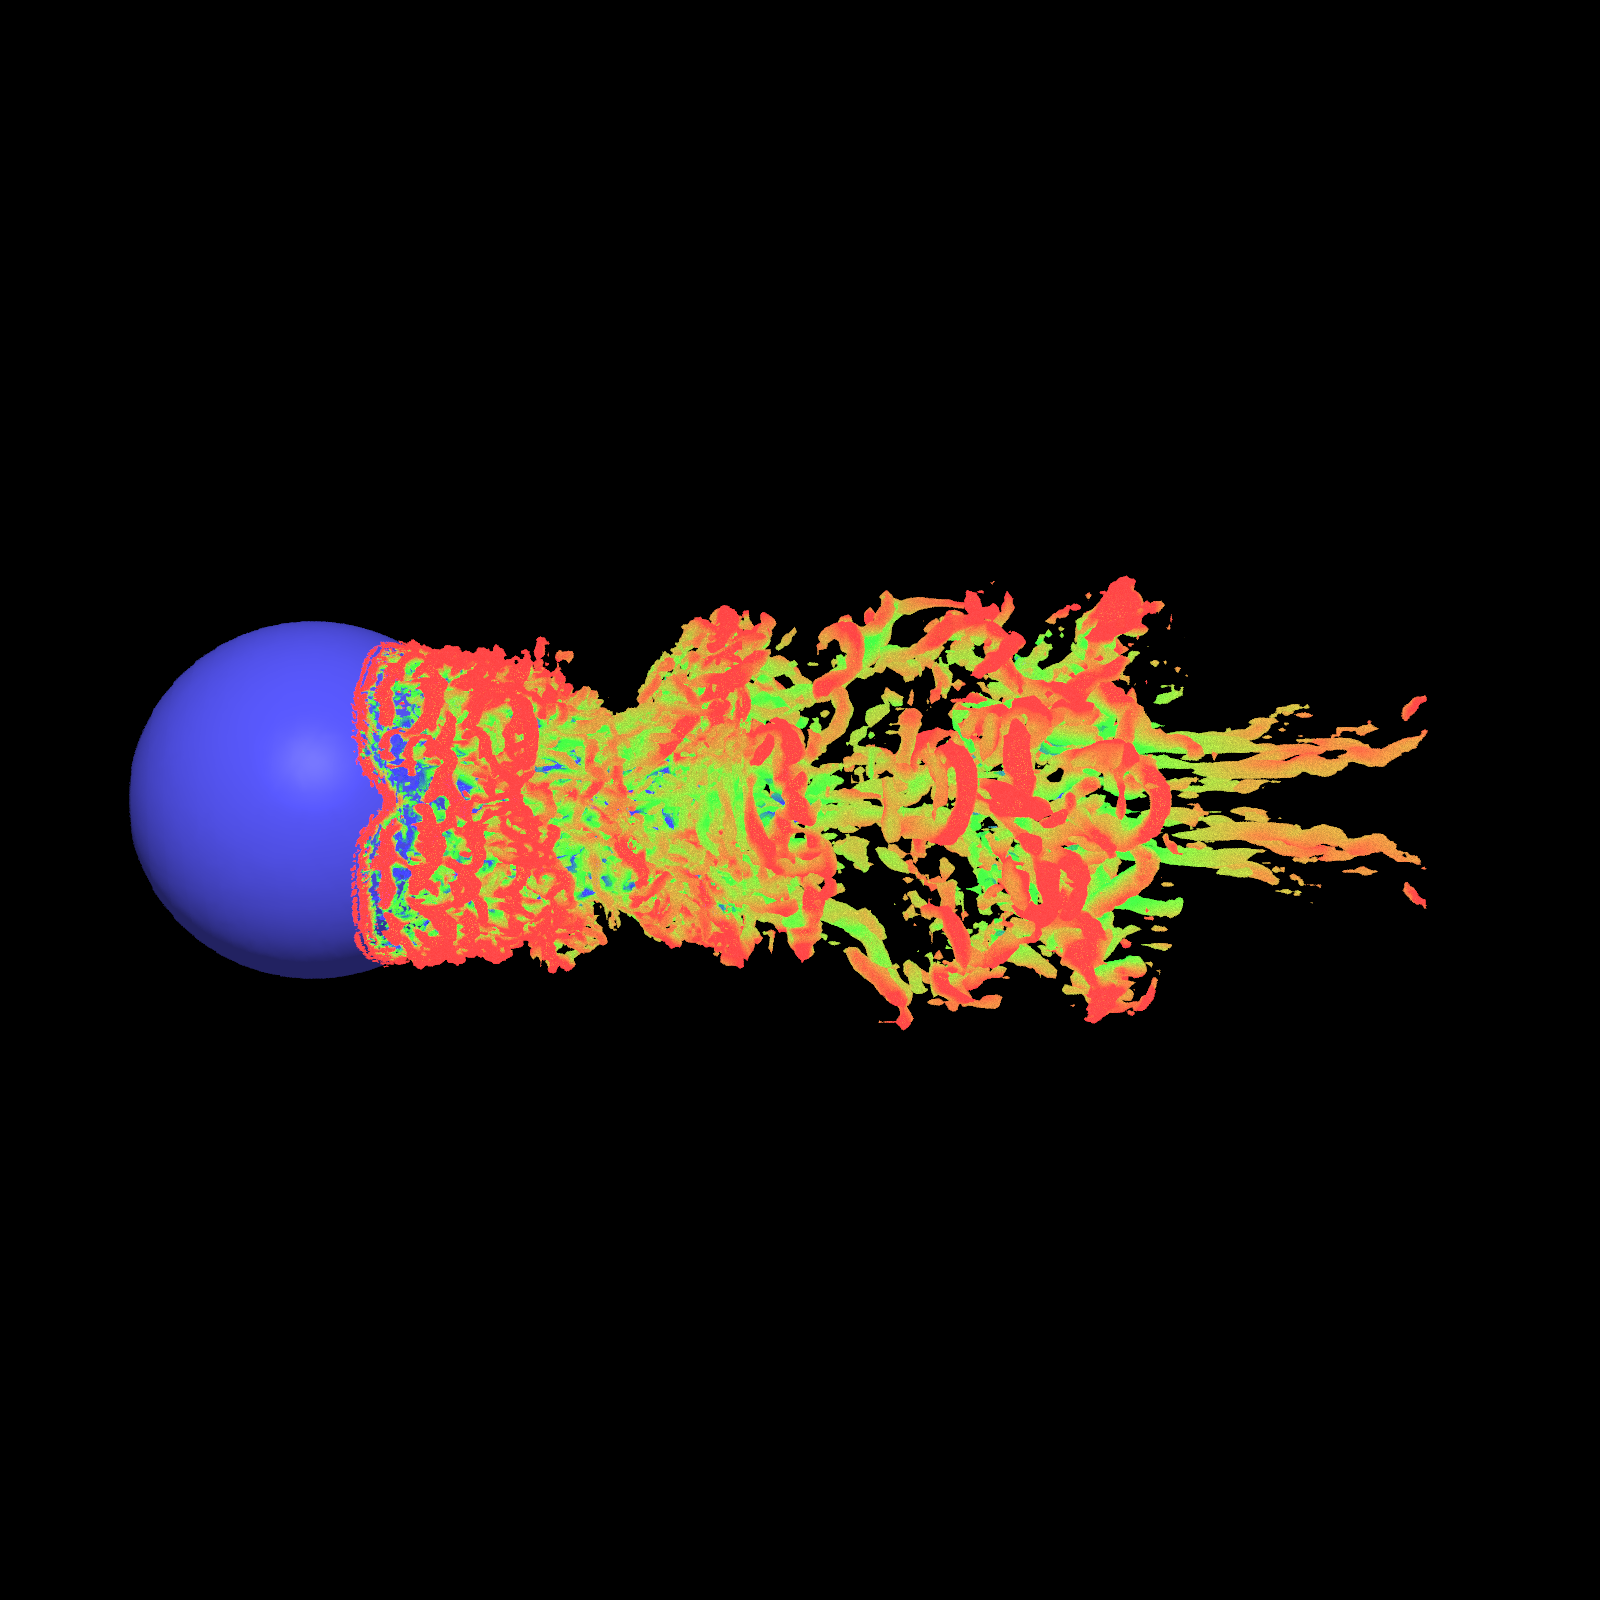
\includegraphics[width = 0.67\linewidth]{images/result_m_b_f.png}
	\caption{Multi-big}
\end{figure}
\begin{figure}[H]
	\centering
	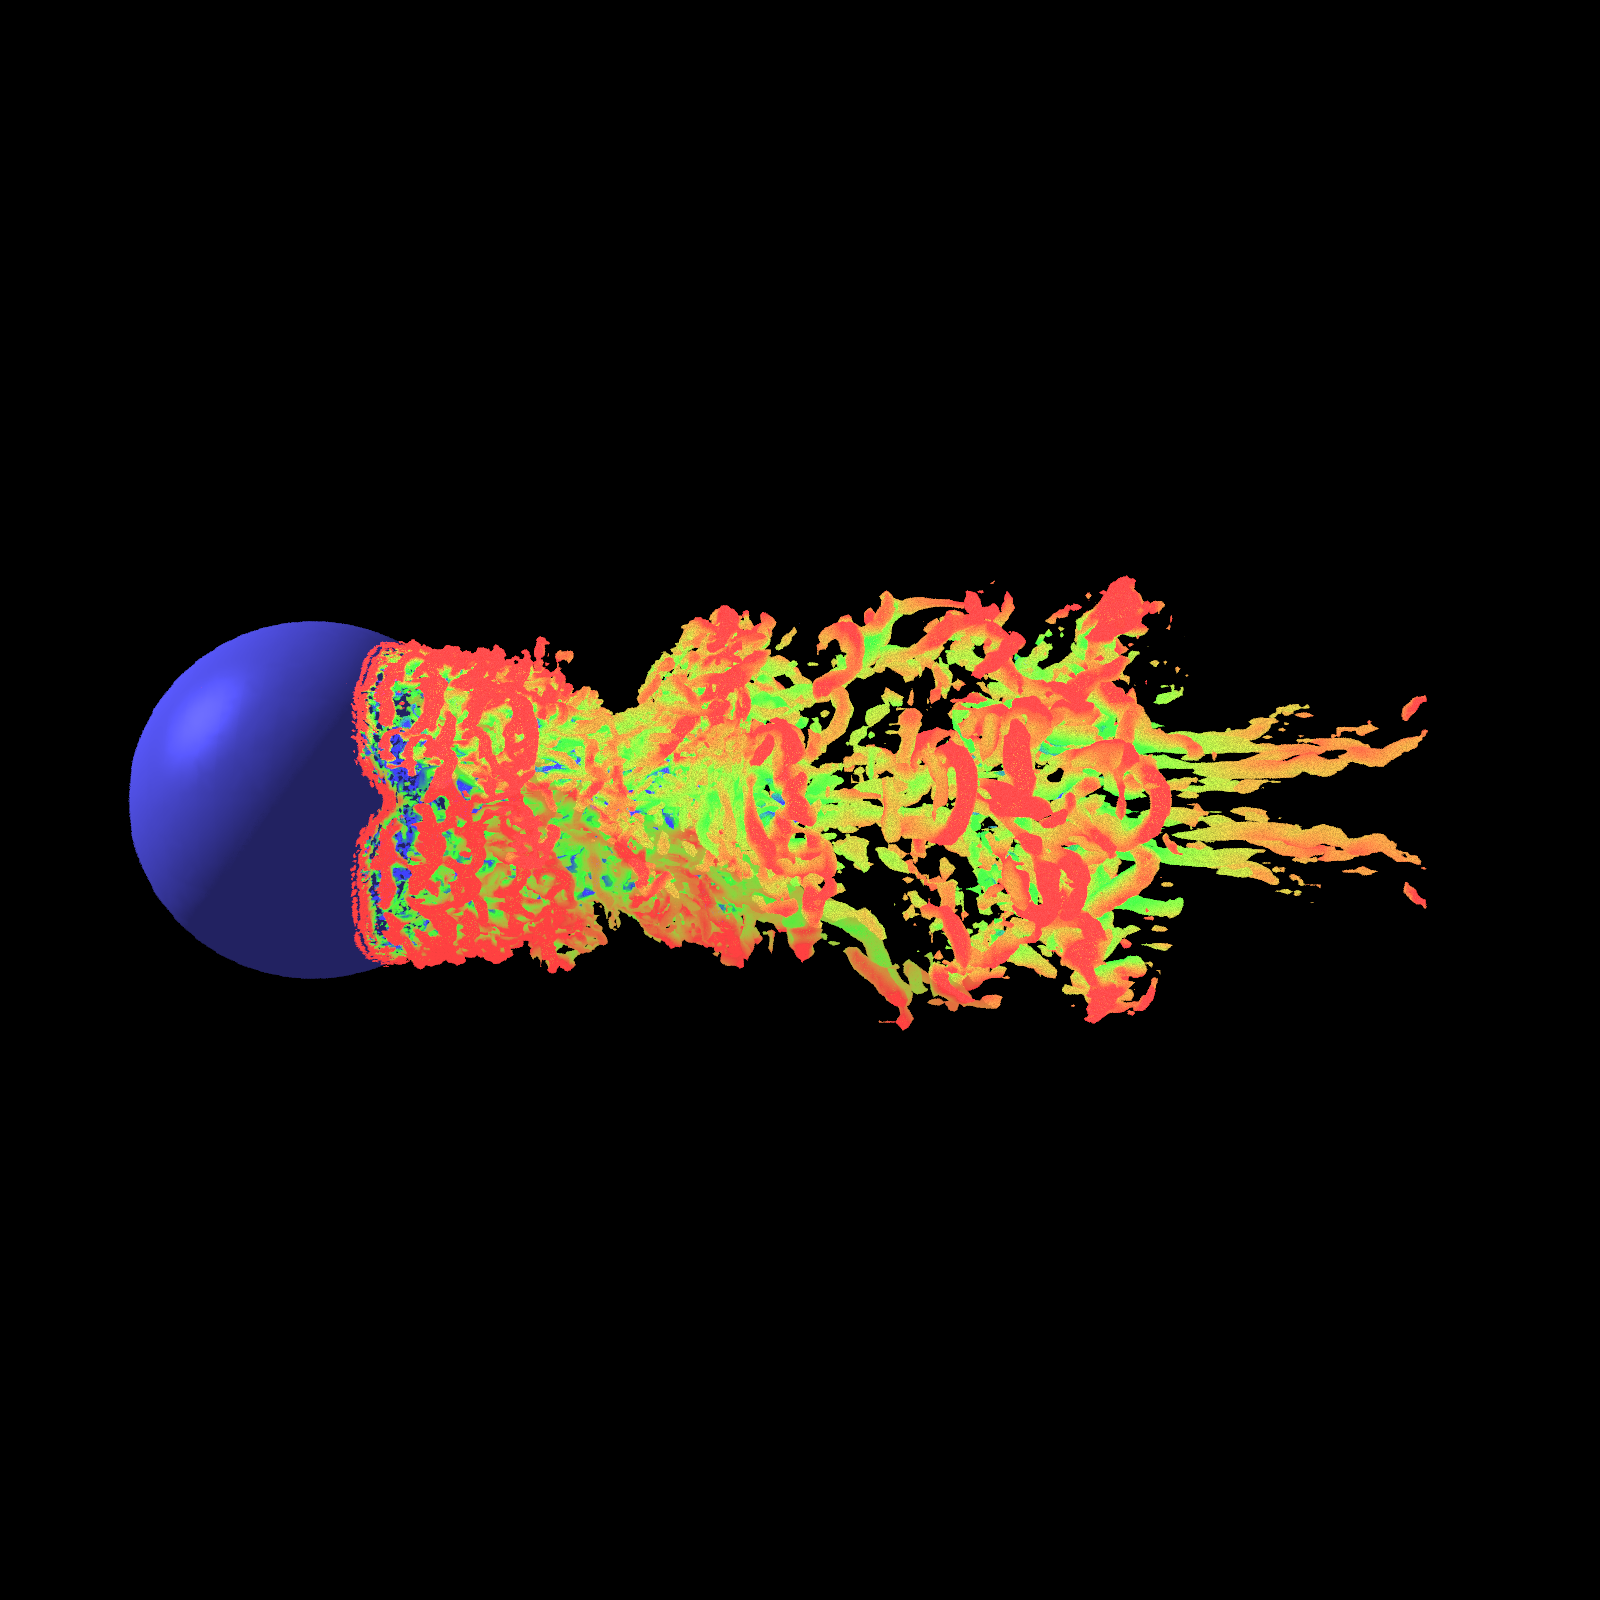
\includegraphics[width = 0.67\linewidth]{images/multi_big_shade.png}
	\caption{Multi-big with shadow}
\end{figure}


\subsection{Single-big Data}


\begin{figure}[H]
	\centering
	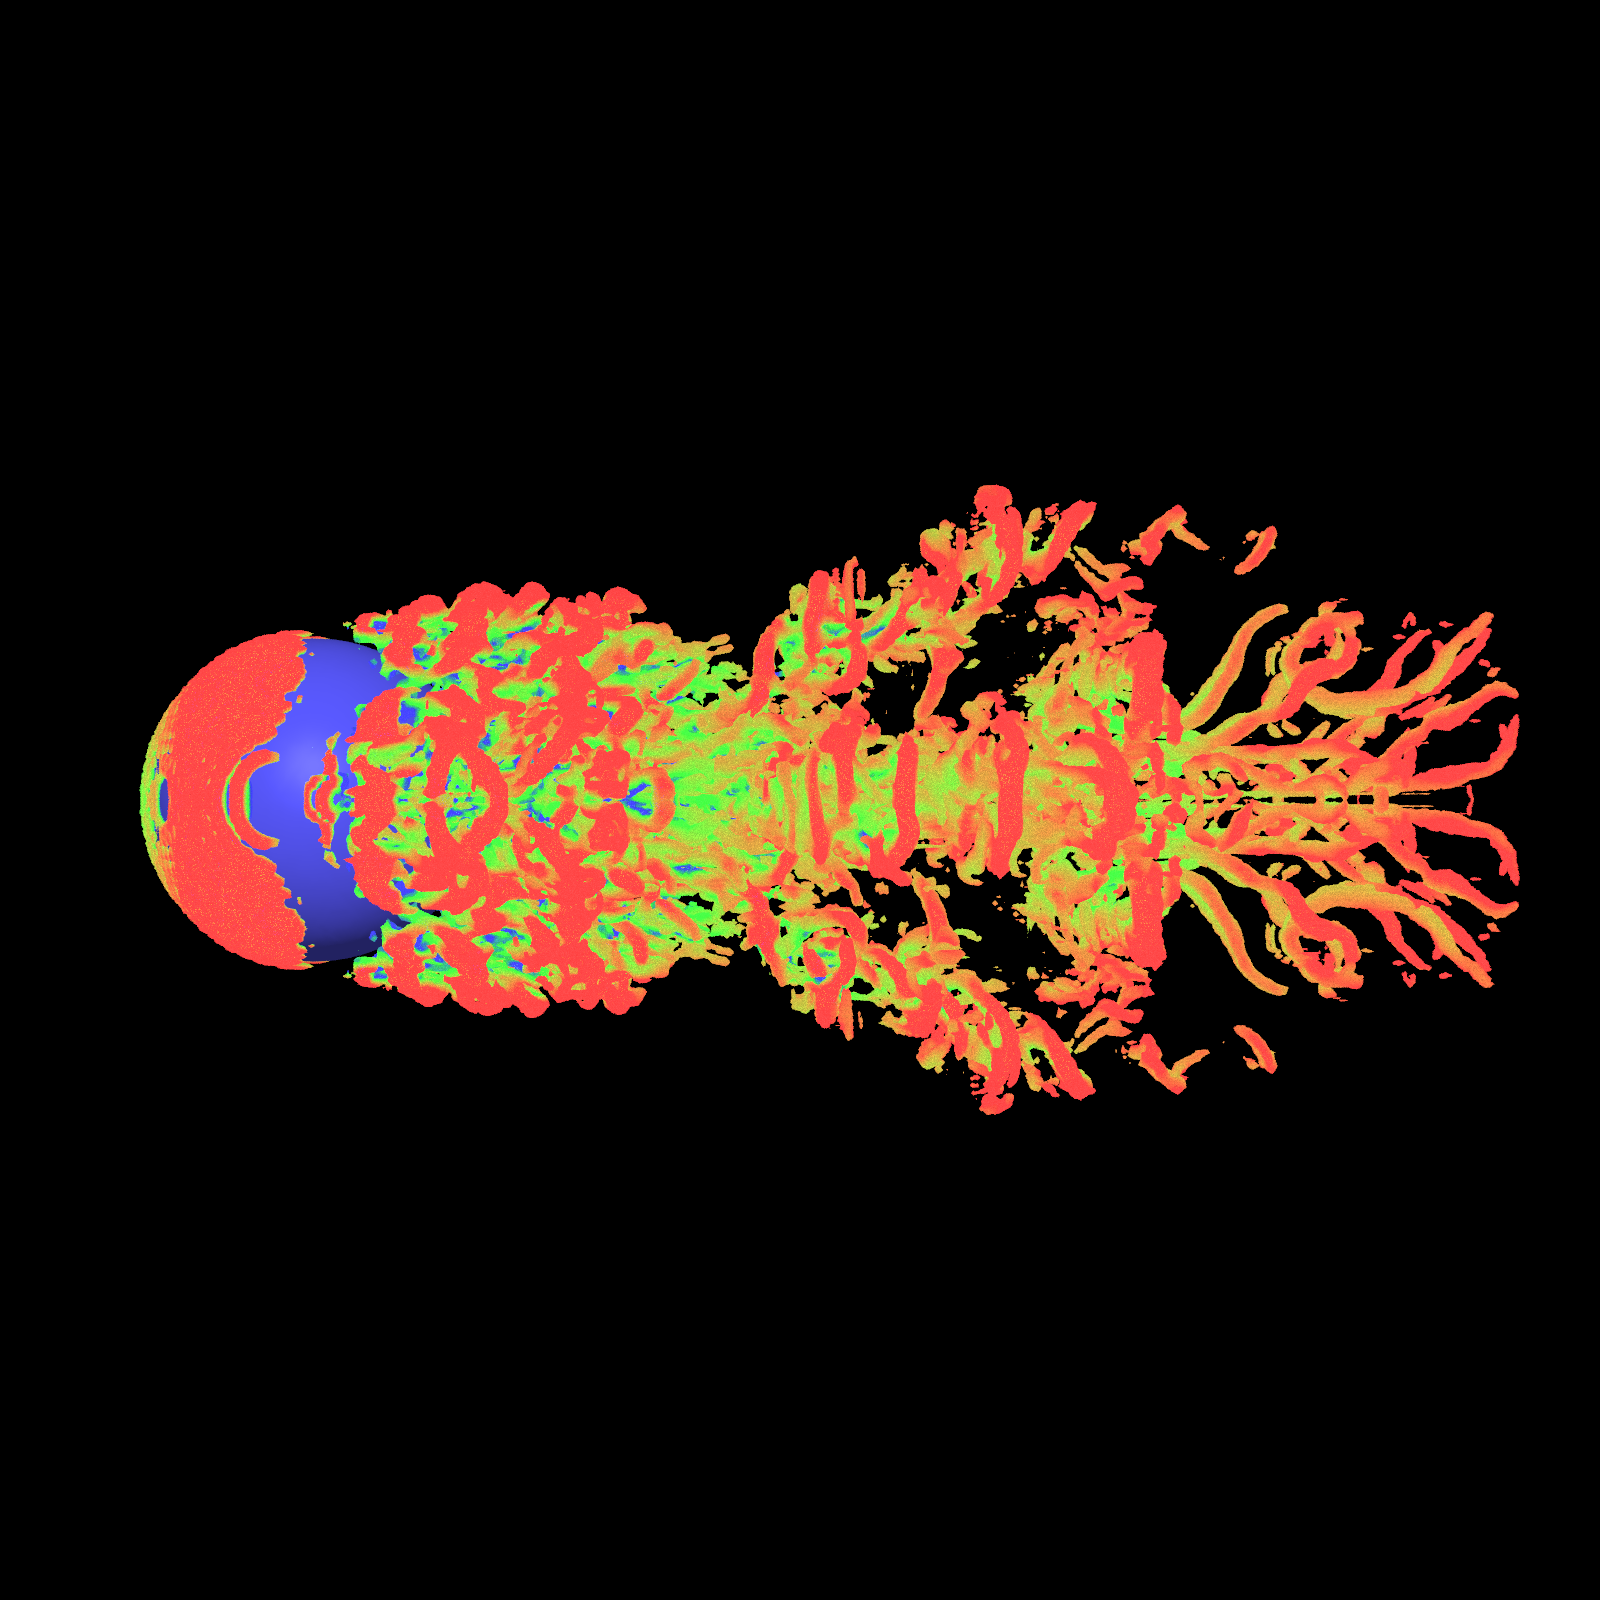
\includegraphics[width = 0.68\linewidth]{images/result_single_big.png}
	\caption{Single-big}
\end{figure}


\section{Group Contribution}


Ren hui: code frame building, VDB, obj data loads in, KD-tree building, front-to-back rendering, (advanced)adaptive sampling, opacity correction, interleaved sampling, Phong lighting implementation.


Li Yian: VDB data processing, interactive transfer function, Advanced adaptive sampling method, interpolation function, gradient calculation, q criterion, few functions in KD tree and BVH.


Song Haiyu: User interface design and implementation, data preprocessing, the advanced BVH, code debugging.


\section{Third libs and references}


The 3rdlibs we used are: openvdb for VDB file io; glfw3, glad, imgui for UI, openmp for multi-threaded acceleration.


The code we referenced: Shanghaitech CG I Homework Assignment 3 and 4, all code is from our own team members' assignments.


The paper we referenced: \\
$[1]$ Wald I, Zellmann S, Usher W, et al. Ray tracing structured AMR data using ExaBricks[J]. IEEE Transactions on Visualization and Computer Graphics, 2020, 27(2): 625-634.\\
$[2]$ Keller A, Heidrich W. Interleaved sampling[C]//Eurographics Workshop on Rendering Techniques. Springer, Vienna, 2001: 269-276.\\
$[3]$ Wald I, Brownlee C, Usher W, et al. CPU volume rendering of adaptive mesh refinement data[C]//SIGGRAPH Asia 2017 Symposium on Visualization. 2017: 1-8.


\end{document}
